
\documentclass[10pt,a4paper]{report}
\usepackage[utf8]{inputenc}
\usepackage[german]{babel}
\usepackage{amsmath}
\usepackage{amsfonts}
\usepackage{amssymb}

\usepackage{listings}
\usepackage[hyphens]{url}
\usepackage{hyperref}
\usepackage{graphicx}

\newcommand{\code}[1]{{\fontfamily{cmvtt}\selectfont #1}}
\newcommand{\HRule}{\rule{\linewidth}{0.1pt}} % Defines a new command for the horizontal lines, change thickness here

\usepackage[left=3cm,right=3cm,top=3cm,bottom=3cm]{geometry}
\begin{document}
% \title{Dokumentation Projekt AAL}
% \author{Tom Nick\\Jonathan Seilkopf\\Niklas Gebauer\\Maximilian Bachl\\Tom Lehmann}
% %\subtitle{Applikationsgruppe}
% \maketitle
% \newpage


\begin{titlepage}


\center % Center everything on the page
 
%	HEADING SECTIONS

\textsc{\LARGE Technische Universität Berlin}\\[2.5cm] % Name of your university/college
\textsc{\Large Projekt AAL}\\[0.5cm] % Major heading such as course name
\textsc{\large Applikationsgruppe}\\[0.5cm] % Minor heading such as course title


%	TITLE SECTION

\HRule \\[0.6cm]
{ \textsc{\Huge Dokumentation}}\\[0.4cm] % Title of your document
\HRule \\[1.5cm]
 
%	AUTHOR SECTION

% \begin{minipage}{0.4\textwidth}
% \begin{flushleft} \large
% \emph{Author:}\\
% John \textsc{Smith} % Your name
% \end{flushleft}
% \end{minipage}
% ~
% \begin{minipage}{0.4\textwidth}
% \begin{flushright} 
% \large
% \emph{Supervisor:} \\
% Dr. James \textsc{Smith} % Supervisor's Name
% \end{flushright}
% \end{minipage}\\[4cm]

% If you don't want a supervisor, uncomment the two lines below and remove the section above
%\Large \emph{Author:}\\
Tom Nick\\
Jonathan Seilkopf\\
Niklas Gebauer\\
Maximilian Bachl\\
Tom Lehmann\\
[3cm] % Your name

%	DATE SECTION

{\large \today}\\[3cm] % Date, change the \today to a set date if you want to be precise


\includegraphics{TU_Logo.pdf}\\[1cm] % Include a department/university logo - this will require the graphicx package

\vfill % Fill the rest of the page with whitespace
\end{titlepage}



\tableofcontents


\chapter{Entwicklerhandbuch}
	\section{Installation}
	Für die vollständige Lauffähigkeit unserer finalen Abgabe, müssen folgende Programme installiert sein:
	\begin{itemize}
		\item \href{http://github.com}{Git (nötig, um den Programmcode von Github herunterzuladen)}
		\item \href{http://www.playframework.com}{Play}
		\item \href{http://nodejs.org}{node.js}
		\item \href{http://www.oracle.com/technetwork/java/javase/downloads/java-se-jre-7-download-432155.html}{Java 1.7} 
		\item \href{http://www.google.de/intl/de/chrome/browser/}{Google Chrome}
	\end{itemize}
	Zum Starten des Projekts muss zunächst das Play-Backend gestartet werden. Das kann getan werden, indem aus dem Projektverzeichnis heraus Play mit
	\code{play run} via Konsole gestartet wird. Nachdem der Server fertig geladen hat, muss die Seite einmalig über die Adresse \url{http://localhost:9000} gestartet werden.
	Bei diesem Aufruf werden die Jiac-Agenten initialisiert und gestartet. Wird die Seite mehrmals über diese URL geladen, werden die Jiac-Agenten mehrfach gestartet. Das kann zu undefiniertem Verhalten führen und sollte deshalb vermieden werden. Nach dem ersten Aufruf, wechselt der Status zu \url{http://localhost:9000/index.html\#/nouser}. Ab sofort reagiert die Wall auf einkommende Nachrichten und ändert ihren Status selbstständig.

	\section{Projektstruktur}
		\subsection{Allgemeiner Aufbau}
			Aus diversen Gründen haben wir uns dazu entschieden das Frontend mit dem, von Google entwickelten, Javascript-Framework AngularJS\footnote{\href{http://angularjs.org/}{http://angularjs.org/}} zu entwickeln. Die komplette Frontendimplementierung befindet sich im Unterordner \code{public/angular/app}. Die Widgets haben wir als Angular-Directives implementiert und diese befinden sich im \code{scripts/directives}-Ordner. Allgemeine Funktionen, welche die gesamte Applikation beziehungsweise den gerade relevanten Teil der Applikation betreffen, werden in den Controllern realisiert. Für häufig genutzte und ausgliederbare Funktionalität, benutzen wir die Services. Ein weiterer zentraler Bestandteil unserer Applikation ist der AngularUI Router\footnote{\href{http://github.com/angular-ui/ui-router}{http://github.com/angular-ui/ui-router}} welcher für die Anzeige und den Wechsel der einzelnen Zustände zuständig ist. Sämtliche visuell relevanten Codeteile befinden sich in dem Unterordner \code{views}.\\\\
			Unser Backend-Code ist im \code{app}-Verzeichnis abgelegt. Die Aufgabe des Backends  besteht im wesentlichen darin, sich um die Kommunikation mit anderen Gruppen des Projekts via Jiac zu kümmern und das Frontend mit Daten zu versorgen. Weiterhin stellt es der Wallapplikation sowie den Mobilgeräten, welche zur Bedienung ebenjener verwendet werden, die Websockets als Kommunikationskanal zur Verfügung.

		\subsection{Frontend}
			\subsubsection{Controllers}
				\paragraph{AuthCtrl}
					Der Auth-Controller ist aktiv, wenn sich die Applikation in einem für die Nutzererkennung relevanten Zustand befindet. Also wenn sie anzeigt, dass gerade eine Erkennung durchgeführt wird oder ein Nutzer als bekannt oder unbekannt identifiziert wurde. Er stellt unter Anderem die Funktionen \code{startTraining} sowie \code{recognizeAgain} bereit, welche über Buttonklicks aufgerufen werden können und die Einleitung eines Trainings- oder Erkennungsprozesses durch das Backend initiieren. Weiterhin stellt er die, für die Anzeige des QR-Codes, relevanten Daten zur Verfügung.
				\paragraph{MainCtrl}
					Der Main-Controller ist in unserer Applikation praktisch der root-Controller. Er wird beim Start als erstes geladen, empfängt \code{ADD\_USER} und \code{REMOVE\_USER} Nachrichten unseres Backends und kümmert sich um die korrekte Zustansänderung der Applikation.
				\paragraph{MobileCtrl}
					Der Mobile-Controller ist auf allen, sich auf der Mobilseite \url{http://localhost:9000/index.html\#/mobile} befindenden, Geräten aktiv. Er wartet auf Nachrichten von der Wall, mit der er gepaired ist und initiiert Zustandsänderungen auf der Angularinstanz, welche auf dem Mobilgerät aktiv ist. Weiterhin sendet er, sofern das \code{modal}-Objekt verändert wurde, das neue Objekt an die Wall, sodass sich die Nutzereingaben auf dem Smartphone direkt im, auf der Wall eingeblendeten, Modal-Fenster verfolgen lassen. Initial befindet das Mobilgerät im Zustand \code{wrapper.mobile.navigation}. Das bedeutet zum einen, dass sowohl der Main- als auch der Mobil-Controller aktiv sind und zum anderen, dass in der Subview der \code{views/mobile.html} die \code{views/widgets/mobile/mobile.navigation.html} geladen wird. Diese bietet direkten Zugriff auf die Core-Features der Applikation vom Mobilgerät aus. Das heißt, man kann ohne auf der Wall navigieren zu müssen, Funktionen wie "`Facebook-Login"' oder "`Add Calendar Entry"' ausführen.
				\paragraph{ModalCtrls}
					Die Modal-Controller sind jeweils aktiv, sobald auf der Wall das entsprechende Eingabemodal für die angeforderte Funktionalität angezeigt wird. Sie kommunizieren mit dem Mobilgerät über Websockets und initiieren dadurch gewünschte Zustandsänderungen im MobileCtrl auf dem Mobilgerät. Die gesamte Funktionalität des ModalSocialCtrl, ist in der finalen Abgabe jedoch nicht erreichbar, da das Posten von anderen Gruppen nicht unterstützt wurde.
				\paragraph{SettingsCtrl}
					Der Settings-Controller ist aktiv, sobald in das Settings-Menü navigiert wurde. Das ist lediglich mit einem Mausklick auf den kleinen Button oben rechts möglich. Für den normalen Betrieb muss das Settings-Menü nicht aufgerufen werden. Es bietet sich aber für Testzwecke an, hier bestimmte Aufgaben manuell auslösen zu können (wie z.B. Facebook-Logout). Da das Settings-Menü für den User nicht sichtbar ist, finden sich hier auch noch Buttons, welche nicht mehr gebraucht werden, oder nicht mehr funktionieren.
				\paragraph{TestCtrl}
					Der Test-Controller simuliert lediglich das Eintreffen von \code{ADD\_USER} bzw. \code{REMOVE\_USER} Nachrichten mit verschiedenen User- und Nite-IDs um die, sich im Main-Controller befindende, Logik zu testen oder einzelne Widgets mit Testdaten zu versorgen. Dazu werden die Nachrichten auf den entsprechenden Kanälen der Websockets versendet.\\
				\HRule
			\subsubsection{Directives}
				\paragraph{Calendar}
					Das Calendar-Widget holt sich seine Daten über einen eigenen "`CALENDAR"'-Channel des Websockets. Außerdem ist hier die Funktionalität zum Hinzufügen eines eigenen Kalendereintrags vorhanden, welche dann das entsprechende Modal öffnet, dessen Controller sich dann um die Kommunikation mit dem Mobilgerät kümmert. Weiterhin benutzen wir Bootstrap\footnote{\href{http://getbootstrap.com/}{http://getbootstrap.com/}} Popovers, um weitere Detailinformationen zu einem Kalendareintrag anzuzeigen. Dazu dient die Funktion \code{showCalendarEntry} welche das Popover öffnet und mit diesem die entsprechenden Daten übergibt. Die zusätzlichen Directives \code{widgetCalendarSmall}, \code{widgetCalendarMiddle} bzw. \code{widgetCalendarBig} dienen lediglich dazu eine modularere, übersichtlichere und elegantere Notation in den HTML-Files zu ermöglichen.
				\paragraph{Debug}
					Das Debug-Widget sollte in der finalen Version selbstverständlich nicht mehr angezeigt werden, da es, wie der Name schon andeutet, lediglich zu Debugzwecken verwendet wird. Es zeigt die Anzahl aller bekannten sowie unbekannten Nutzer und die drei zuletzt erkannten Gesten an. Weiterhin zeigt es das für die Gesichtserkennung verwendete Bild, sowie User- und NiteID des jeweiligen Nutzers an. 
				\paragraph{Fair}
					Das Messe-Widget, zeigt lediglich hart codierte Daten an. Diese werden im in der \code{views/fair.html} übergeben. Logik zum holen von Daten ist noch nicht implementiert, da andere Gruppen dieses Szenario nicht unterstützen, ließe sich aber mit geringem Aufwand aus einem der anderen Widgets ableiten. 
				\paragraph{Mail} 
					Das Mail-Widget holt sich seine Daten über einen eigenen "`MAIL"'-Channel des Websockets. Der Rest der Funktionalität ist beinahe Äquivalent zum Calendar-Widget.
				\paragraph{Widget}
					Das Widget-Directive ist eine Art Wrapper dem wir die Daten für das eigentliche Widget sowie einen Widget-Type übergeben. Es fügt dann einen HTML-Tag mit typspezifischen CSS-Klassen um den eigentlichen Widget-Tag herum ein. Das hat den Vorteil, dass man beim Hinzufügen von Widgets in der \code{views/main.html} weniger beachten muss.
				\paragraph{Maps}
					Das Maps-Widget zeigt Google-Maps an. Man kann seinen Standort bestimmen und dann Dinge sehen, die es in der Nähe zu erkunden gibt. Das Google-Maps ist in der finalen Version allerdings nicht mehr enthalten, da wir lieber auf andere Widgets zurückgegriffen haben. Es lässt sich allerdings bei Bedarf wieder aktivieren.
				\paragraph{News}
					Das News-Widget wartet lediglich auf Daten in dem "`NEWS"'-Channel des Websockets und bietet eine Funktion um einen Newsbeitrag in einem Modal detailiert anzuzeigen.
				\paragraph{Personal}
					Das Personal-Widget zeigt persönliche Informationen des Users an. Diese holt es sich über den "`FACEBOOK"'-Channel des Websockets. Weiterhin kann man sich den QR-Code, welcher auf die Mobilseite verlinkt mit einem Modal in groß anzeigen lassen.
				\paragraph{Social-Comparison (Social-Graph)}
					Das Social-Comparison Widget füllt den Bildschirm komplett aus und visualisiert die Gemeinsamkeiten zwischen zwei Personen. So werden etwa gemeinsame Vorlieben für Musik, gemeinsame Freunde, aber auch gemeinsame Sportarten gefiltert und präsentiert. Die verschiedenen Gemeinsamkeiten sind außerdem semantisch gruppiert, das heißt es werden Filme, Freunde etc. getrennt dargestellt. Es wird mit einer speziellen Geste geöffnet und kann nur angezeigt werden, wenn zwei bekannte Nutzer vor der Living Wall stehen.
				\paragraph{Social}
					Das Social-Widget zeigt dem User aktuelle Facebook-Posts aus seinem Facebookstream an. Die Daten bekommt es aus dem "`SOCIAL"'-Channel. Weiterhin stellt es die Möglichkeit zur Verfügung detailierte Informationen zu einem Post, wie Anzahl an Likes und Kommentaren, sowie die ersten Kommentare in einem Popover anzuzeigen. Auch das Liken eines Facebookposts ist möglich.
				\paragraph{To Do}
					Das To-Do-Widget zeigt die ToDos an, welche auf dem "`TODO"'-Channel ankommen. \code{showTodo} kümmert sich hier um die Anzeige detailierter Informationen zu einem ToDo.\\
				\HRule
			\subsubsection{Services}
				\paragraph{CSS-Service}
					Hier wird ein Array von CSS-Klassen erstellt, was für jedes Widget eine eigene CSS-Klasse erstellt, die die Farbendarstellung im Widget beschreibt.
				\paragraph{Radial-Service}
					Der Radial-Service ist ein zentraler Bestandteil unserer Applikation. Er stellt das Menü zur Verfügung. Das Menü ist insofern parametrisiert, als dass es nur die tatsächlich vorhandenen Widgets einbezieht und in den Submenüs auch immer nur so viele Auswahlmöglichkeiten anzeigt, wie Daten verfügbar sind. In der anfangs notierten \code{KEYMAPPING}-Variable werden die Tasten deklariert, die der Service für bestimmte Aktionen erwartet. Die Tastendrücke werden im Backend ausgelöst. Das hat den großen Vorteil, dass wir im Frontend direkt auf keypress-Events reagieren können und einige von uns benutzte Elemente, wie beispielsweise Modals, bereits das von uns gewünschte Verhalten (z.B. das Schließen bei Escape-Tastendruck) mitbringen.\\
					Das Verhalten und die Funktionsweise des Menüs lassen sich recht einfach erschließen, indem man den switch-case-Block am Ende des Codes nachvollzieht.
				\paragraph{Social-Comparison-Service}
					Der Social-Comparison-Service ist das Backend für den Social Graph. Hier wird auf das Facebook-API zugegriffen. Durch das modulare Design hat man die Möglichkeit, noch weiter Daten von Facebook herunterzuladen und im Social-Graph zu visualisieren. Das Hinzufügen einer neuen Kategorie benötigt sonst keinen weiteren Aufwand, denn der graphische Teil passt sich dynamisch an die neuen Daten an, die im Source-Code spezifiziert wurden.\\
					Das konkrete Vorgehen ist folgendes: Zuerst wird der Access-Token für Facebook über \texttt{setToken} für den Service gesetzt. Dann werden die Namen der beteiligten Personen an die Funktion \texttt{compare\-Two\-Persons} übergeben. Anschließend werden alle relevanten Daten von Facebook geholt. Diese Daten werden anschließend gruppiert, auf Gemeinsamkeiten überprüft und zuletzt werden doppelte Datensätze noch gefiltert und Verworfen.\\
					Das JSON-Objekt wird als Antwort an das Frontend übergeben, weches die Daten dann visualisiert.
				\paragraph{Transmit-Text-Service}
					Der Transmit-Text-Service stellt verschiedene Methoden zur Daten- bzw. Textübertragung via Websocket zur Verfügung. Dabei verwenden die Funktionen welche "`Text"' im Funktionsnamen enthalten stets auf irgendeine Weise die MobileID für den Über\-trag\-ungs\-chan\-nel, sodass hier nur gepairte Geräte welche die gleiche MobileID verwenden Nachrichten bekommen. Funktionen mit "`Data"' im Funktionsnamen werden benutzt um Daten an Widgets zu senden bzw. diese zu empfangen.
				\paragraph{Websocket-Service}
					Der Websocket-Service wird lediglich vom Transmit-Text-Service benutzt und stellt diesem Funktionen zum Hinzufügen bzw. entfernen von sogenannten Listenern, sowie zum Senden von Nachrichten zur Verfügung.
				\paragraph{Widget-Data-Service}
					Der Widget-Data-Service kümmert sich zum einen um den FB-Login-Status und das Holen und Übertragen der Facebookdaten an das Social-Widget und zum anderen, stellt er die Liste, der über das Menü ansteuerbaren, Widgets inklusive deren Sockets etc. sowie deren Farben zur Verfügung.\\
					\HRule
			\subsubsection{Styles}
				\paragraph{responsive}
					In der responsive.css wird für verschiedene Anzeigeweiten die body-Schriftgröße festgesetzt, sodass die \code{em}-Einheit, welche sich nach der body-Schriftgröße richtet ebenfalls angepasst wird. Außerdem werden für alle von uns verwendeten Bootstrap-Komponenten, die \code{px}-Werte mit passenden \code{em}-Werten überschrieben.\\
					\HRule
			\subsubsection{Views}
				\paragraph{Loading}
				\paragraph{New}
				\paragraph{Train}
				\paragraph{Unknown}
				\paragraph{Userselect}
				\paragraph{Welcome}


	

    \newpage
    \subsection{Backend}
    Der Code für das Backend befindet sich im \code{app}-Verzeichnis.
         \subsubsection{JIAC}
        Zur Kommunikation mit den anderen Projekt-Gruppen benutzen wir das Agentenframework JIAC, über das Nachrichten gesendet werden, die für das Zusammenwirken der einzelnen Teilprojekte nötig sind. Die JIAC-Konfigurationsdatei befindet sich im Verzeichnis \code{aal/conf/jiac.xml}. Während sich die Implementierung der Beans im Verzeichnis \code{jiac/beans} befindet. Alle Beans erben von der Klasse \code{AbstractCommunicatingBean}, um die Modellierung der Beans möglichst weit zu vereinheitlichen und zu vereinfachen. Die Kommunikation läuft über folgende vier Agenten, welche zu dem
        ApplicationNode gehören:
        \paragraph{Gesture Agent}
            Agent zur Kommunikation mit der Gesten und Personenerkennung.
        \paragraph{SocialMedia Agent}
            Agent zur Beschaffung von Daten aus
            SocialMedia Plattformen wie z.B. Facebook, aus der Datenbank.
        \paragraph{Information Agent}
            Agent zur Beschaffung von News und Verwaltung
            von ToDo's aus der Datenbank.
        \paragraph{Communication Agent}
            Agent zur Beschaffung und Verwaltung von
            Mails und Kalender.
        \paragraph{Beans}
        Im Folgenden nun eine Auflistung aller Beans mit kurzer Beschreibung,
        wofür sie gebracht werden:
        \begin{itemize}
        \item Gesture Bean: \\
            Sendet Nachrichten zum starten des Trainings einer neuen Person und zum erneuten erkennen einer Person, falls diese nicht richtig erkannt wurde.\\
            Außerdem Empfängt er Gesten, die über virtuelle Tastendrücke Aktionen im Frontend auslösen und Nachrichten zur Benutzererkennung.
        \item Todo Bean: \\
            Fordert ToDo's des aktuellen Benutzers an und leitet die empfangenen Daten über einen Websocket an das Frontend weiter.\\
            Außerdem bietet er die Möglichkeit Nachrichten zu versenden für das Löschen eines existierenden ToDo's und das erstellen eines neuen ToDo's.
        \item News Bean: \\
            Fordert aktuelle Nachrichten an und leitet die empfangenen Daten an das Frontend weiter über einen Websocket.
        \item Calendar Bean: \\
            Fordert Kalenderdaten des aktuellen Benutzers an und leitet die empfangenen Daten über einen Websocket an das Frontend weiter. Außerdem bietet er die Möglichkeit einen veränderten Kalendereintrag in der Datenbank zu speichern.
        \item Mail Bean: \\
            Fordert Mails des aktuellen Benutzers von der Datenbank an und leitet die empfangenen Daten über einen Websocket an das Frontend weiter.\\
            Zusätzlich bietet er die Möglichkeit des Versendens von Mails.
        \item Facebook Bean: \\
            Fordert Facebook-Profildaten des aktuellen Benutzers an. Die Nachricht enthält entweder ein gültiges access Token, wenn sich der Benutzer neu bei Facebook eingeloggt hat, oder das Feld für das Token bleibt leer. In diesem Fall wird das letzte gespeicherte Accesstoken von der Datenbank verwendet um die Daten zu beschaffen. \\
            Die empfangenen Daten werden über einen Websocket an das Frontend weitergeleitet.
        \end{itemize}
	\section{Erweiterung}
		\subsection{Widget hinzufügen}
			Zum Hinzufügen eines Widgets müssen folgende Dateien geändert werden:
			\begin{itemize}
				\item{} scripts/services/widget-data.service.js
				\item{} index.html
				\item{} views/main.html 
			\end{itemize}
			Und in den folgenden Ordnern die entsprechenden Dateien für das Widget neu erstellt werden:
			\begin{itemize}
				\item{} scripts/directives/
				\item{} views/widgets/
				\item{} views/modals/ (falls benötigt)
			\end{itemize}
			In der \code{widget-data.service.js} befinden sich am Ende der Datei die beiden Arrays \code{widgets} und \code{colors}. Dort muss jeweils der entsprechende Eintrag für das neue Widget hinzugefügt werden. Dabei ist zu beachten, dass der neue Eintrag an der Position in die Arrays eingetragen werden muss, an der das Widget im Quellcode der \code{main.html} notiert ist, um eine korrekte Funktion des Auswahlmenüs zu gewährleisten.\\\\
			In der \code{index.html} muss die Javascript Datei, welche sich im \code{scripts/directives}-Ordner befinden sollte, für das neue Directive eingetragen werden.\\\\
			Das neue Widget muss, um tatsächlich angezeigt zu werden noch in der \code{main.html} notiert werden. Dabei hängt die Postition von der Stelle an der es im Quellcode steht ab. Dazu müssen entweder andere Widgets entfernt werden oder deren Größe angepasst werden. Das kann über das Zuweisen der entsprechenden \code{row-md}-CSS-Klasse erreicht werden. 
		\subsection{Widget ändern}
			\subsubsection{Position ändern}
				Um die Position des Widgets zu ändern, müssen folgende Dateien angepasst werden:
				\begin{itemize}
					\item{} scripts/services/widget-data.service.js
					\item{} views/main.html 
				\end{itemize}
				In welcher Reihenfolge und Größe die einzelnen Widgets angeordnet sind, wird vollständig in der \code{main.html} beschrieben. Sie werden in drei Spalten angezeigt. Die Höhe eines jeden Widgets (in Grideinheiten) wird über die \code{col-md}-Klasse angegeben. Jede Spalte hat eine Gesamthöhe von acht Grideinheiten. Möchte man jetzt beispielsweise ein Widget der dritten Spalte mit einem Widget der ersten Spalte vertauschen, dann muss man darauf achten, dass die Gesamthöhe der Widgets in der ersten sowie der dritten Spalte auch nach dem Tausch acht beträgt.\\\\
				Anschließend müssen die Arrayeinträge der vertauschten Widgets in den Arrays \code{widgets} und \code{colors} in der \code{widget-data.service.js} so verschoben werden, dass die Einträge in den Arrays wieder die gleiche Reihenfolge aufweisen, wie die in der \code{main.html} notierten Widgets. Ist dies nicht der Fall, kann es zu Problemen mit dem Menü kommen.
			\subsubsection{Logik ändern}
				Um die Logik eines Widgets x zu ändern (z.B. weil sich das Datenformat ändert), müssen folgende Dateien angepasst werden:
				\begin{itemize}
				\item{} scripts/directives/widget.x.js
				\end{itemize}
			\subsubsection{Darstellung ändern} 
				Um die visuelle Darstellung eines Widgets x zu ändern, müssen folgende Dateien angepasst werden:
				\begin{itemize}
					\item{} views/widgets/x/*
				\end{itemize}
				Die jeweiligen \code{small}, \code{middle} und \code{big}-Dateien eines Widgets visualisieren jeweils ein Rechteck mit bestimmten Abmessungen im Bootstrap-Grid. Sollen beispielsweise neue Felder eines Kalendareintrags angezeigt werden, dann muss zunächst entschieden werden, ob sie in allen drei Darstellungsgrößen visualisiert werden sollen oder nur in einer Teilmenge. Die geeignete Darstellung kann dann in den entsprechenden HTML-Dateien notiert werden. Soll die Zusammensetzung oder Reihenfolge der unterschiedlichen Rechtecke des Widgets verändert werden, muss das in der \code{widget.x.html} erledigt werden.
		\subsection{Widget entfernen}
			Um ein Widget nicht mehr anzuzeigen, müssen folgende Dateien geändert werden:
			\begin{itemize}
				\item{} scripts/services/widget-data.service.js
				\item{} views/main.html
			\end{itemize}
			Das zu entfernende Widget muss zum einen aus der \code{main.html} entfernt werden und die anderen, in dieser Spalte dargestellten Widgets, müssen gegebenenfalls in ihrer Höhe, über die Zuweisung einer anderen \code{col-md}-Klasse, angepasst werden.\\\\
			Zum anderen müssen noch die entsprechenden Einträge in den Arrays \code{widgets} und \code{colors} in der \code{widget-data.service.js} entfernt werden.



\chapter{Nutzeranleitung}
Die Living Wall kann mit Gesten, per Touchscreen und via Smartphone gesteuert werden. Da die Bildschirme, auf denen die Living Wall läuft allerdings in der Regel sehr groß sind, raten wir dazu, alle Eingaben bei circa 2 Metern Abstand von der Wand mit Gesten und einem Smartphone vorzunehmen. Die folgende Anleitung wird dementsprechend auch ausführlicher auf die Gesten- und Smartphonesteuerung eingehen.

	\section{Gesten}
	Vorab seien die Gesten erklärt, mit denen die Wall bedient werden kann. Für genauere Erläuterungen zur Gestenerkennung und -ausführung sei auf die Dokumentation der Gestengruppe verwiesen. Um die Living Wall ordnungsgemäß bedienen zu können, sollten die User möglichst frontal zu dieser stehen.
		\subsection{Einhändige Gesten}
		Folgenden Gesten können je nach Belieben des Nutzers entweder mit der linken oder mit der rechten Hand ausgeführt werden:
		\subsubsection{Enter}
		Die Enter-Geste dient zur Bestätigung einer Auswahl. Sie kann als ein Knopfdruck oder Mausklick verstanden werden.\\
Um die Geste auszulösen, muss eine Hand für einen kurzen Moment vom Körper in Richtung Living Wall geführt und wieder zurückgezogen werden. Ein Arm wird also kurz nach vorne hin gestreckt und wieder gebeugt - wie zum Beispiel beim Knopfduck im Fahrstuhl.
		\subsubsection{Vierwege-Tabbing}
		Es ist möglich, einen Tab nach oben, unten, links oder rechts auszuführen. Dazu wird eine Hand parallel zur Living Wall in eine der vier Richtungen bewegt und wieder zurück gezogen.\\
Das Zurückziehen der Hand unterscheidet das Tabbing vom Scrolling.
		\subsubsection{Scrolling}
		Scrolling ist in der horizontalen Ebene, also nach links und nach rechts, möglich. Um zu scrollen muss eine Hand parallel zur Living Wall in die gewünschte Richtung geführt und dort gehalten werden, solange gescrollt werden soll. Sobald die Hand zurück gezogen wird, endet das Scrolling.
		\textit{Hinweis: Das Scrolling wird in der momentanten Version der Living Wall nicht benötigt, da alle Anzeigen so angepasst sind, dass sie auf dem ganzen Bildschirm lesbar sind, ohne verschoben werden zu müssen. Das Rechts- oder Linksscrollen löst deswegen die selbe Aktion wie ein Links- oder Rechtstab aus.}
		\subsection{Zweihändige Gesten}
		Folgende Gesten müssen immer mit beiden Händen ausgeführt werden:
		\subsubsection{Gestenerkennung ein-/ausschalten}
		Manchmal ist es erwünscht, beliebige Bewegungen vor der Wand ausführen zu können, ohne dabei eine Aktion auszulösen. Für diesen Fall kann die Gestenerkennung ab- und wieder eingeschaltet werden. \\
Um die Gestenerkennung vorübergehend zu blockieren, müssen beide Arme gleichzeitig in Richtung Living Wall ausgestreckt und wieder zurückgezogen werden. Es handelt sich also um ein 'Enter' mit beiden Händen gleichzeitig.\\
Um die Gestenerkennung wieder zu aktivieren, muss ein weiteres Mal ein 'Enter' mit beiden Händen gleichzeitig ausgeführt werden.
		\subsubsection{Menü öffnen}
		Das Menü kann in der Hauptansicht geöffnet werden, indem beide Hände gleichzeitig nach Außen vom Körper weggeführt und wieder zurückgezogen werden. Es handelt sich also um einen gleichzeitigen Tab nach rechts mit der rechten Hand und Tab nach Links mit der linken Hand.
		\subsubsection{Escape}
		Die Escape-Geste wird verwendet, um das gesamte Menü zu schließen. Um sie auszulösen, müssen beide Hände gleichzeitig nach oben und wieder zurück geführt werden. Es handelt sich dementsprechend um ein Tab nach oben mit beiden Händen gleichzeitig.
		\subsubsection{Social-Graph-Ansicht öffnen}
		Wenn sich mehrere bekannte Nutzer vor der Wall befinden, kann mit dieser Geste in die Social-Graph-Ansicht, in der Gemeinsamkeiten der Nutzer angezeigt werden, gewechselt werden. Dazu mussen beide Hände gleichzeitig parallel zur Living Wall nach rechts und wieder zurück geführt werden. Die Geste kann als gleichzeitiges Tabben nach rechts mit beiden Händen verstanden werden.
		\subsubsection{User-Auswahl anzeigen}
		Wenn sich mehrere Nutzer vor der Living Wall befinden, kann ausgewählt werden, welcher Nutzer der Hauptnutzer sein soll, dessen Informationen in der Hauptansicht mit diversen Widgets angezeigt werden.\\
Um zur User-Auswahl zu gelangen, müssen beide Hände gleichzeitig parallel zur Living Wall nach links und wieder zurück geführt werden. Die Geste kann als gleichzeitiges Tabben nach links mit beiden Händen verstanden werden.

	\section{Benutzung}
	Im folgenden werden die verschiedenen Nutzungsmöglichkeiten und die genaue Bedienung der Living Wall erklärt. Die verwendeten Gesten richten sich nach der vorherigen Auflistung unter Punkt \textit{2.1}, wobei das 'Vierwege-Tabbing' je nach Richtung als 'Tab nach rechts', 'Tab nach links', 'Tab nach oben' und 'Tab nach unten' beschrieben wird.
		\subsection{Ein Nutzer}
		\subsubsection{Hauptansicht (ohne User)}
		Solange sich kein User im Sichtfeld der Kinectkamera der Living Wall befindet, wird ein schlichter weißer Bildschirm angezeigt: \\
		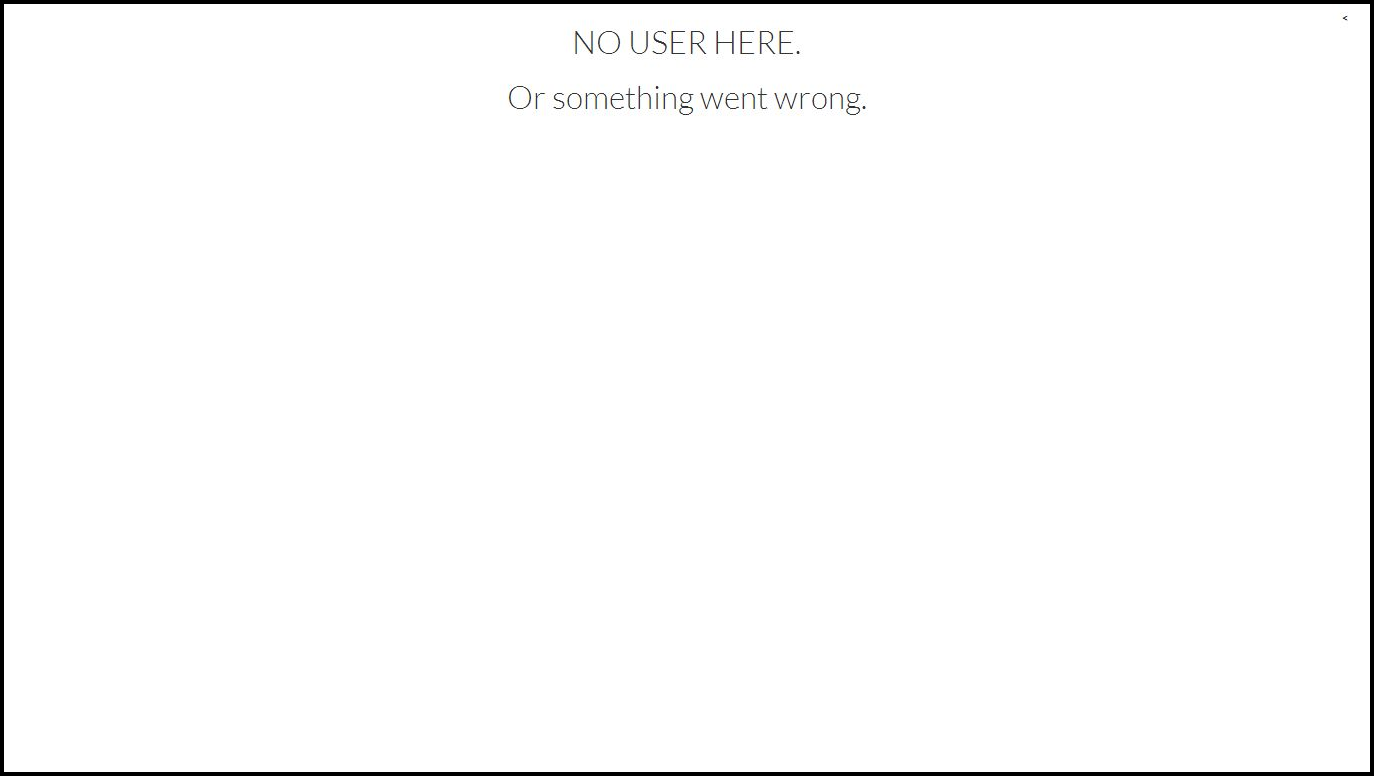
\includegraphics[scale=0.31]{NoUser} \\
		\textit{Hinweis: Sollte dieser Bildschirm nicht verschwinden, obwohl ein oder mehrere Benutzer das Sichtfeld der Kamera betreten, deutet dies darauf hin, dass entweder die Kinectkamera nicht richtig angeschlossen bzw. ausgerichtet ist, nicht alle Komponenten der Living Wall (Gesichtserkennung, Gestenerkennung, Datenbank) oder die JIAC-Agenten nicht richtig gestartet wurden.}
		\subsubsection{Nutzererkennung}
		Sobald nun ein Nutzer das Sichtfeld der Kinectkamera betritt, wird der Erkennungsprozess gestartet:\\
		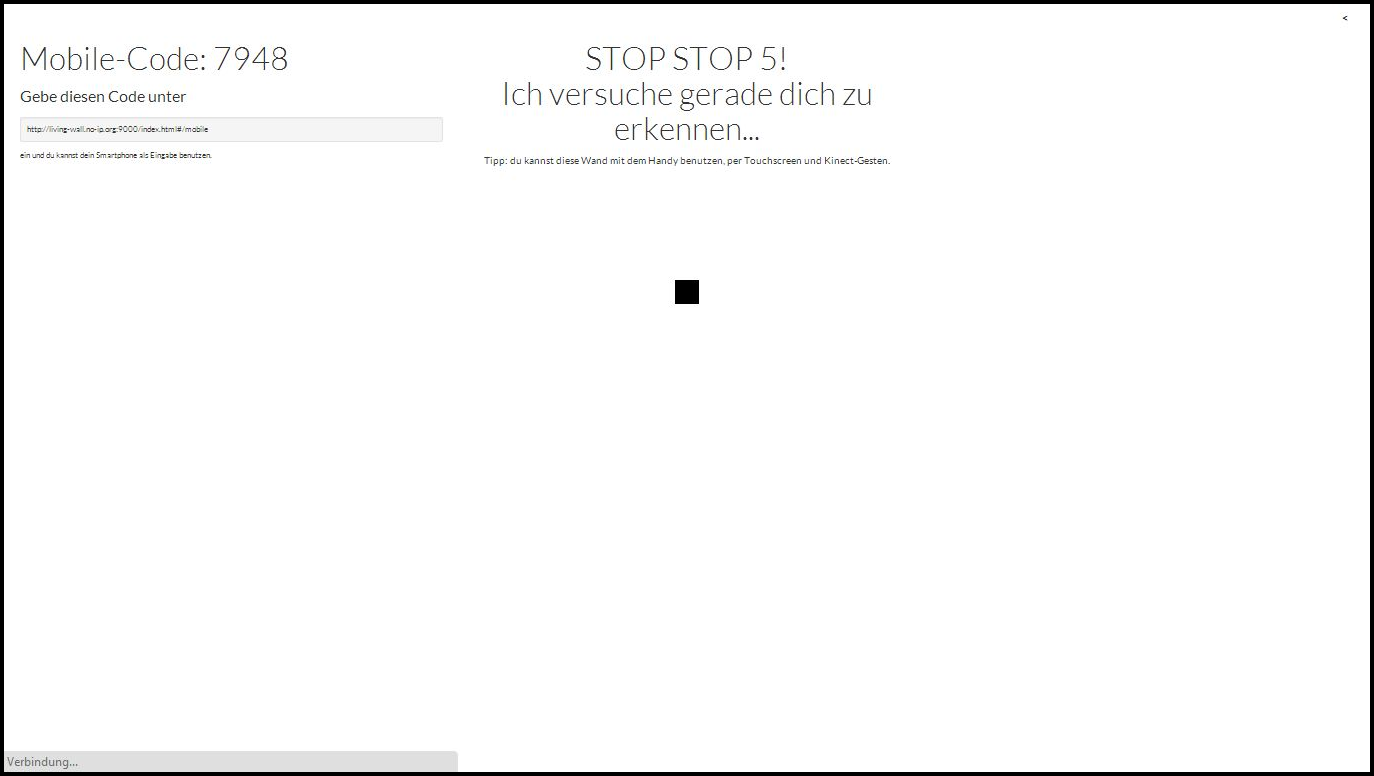
\includegraphics[scale=0.31]{Erkennung}\\Während dieser Bildschirm angezeigt wird, sollte der Nutzer möglichst in ungefähr zwei Metern Abstand frontal zur Kamera stehen und in deren Linse blicken.\\
Je nachdem, ob der Nutzer von der Kinectkamera erkannt wird oder nicht, öffnen sich verschiedene Dialoge.
		\subsubsection{Unbekannter Nutzer}
		Sollte der Nutzer von der Gesichtserkennung als unbekannt eingestuft werden, erscheint folgender Bildschirm:\\
		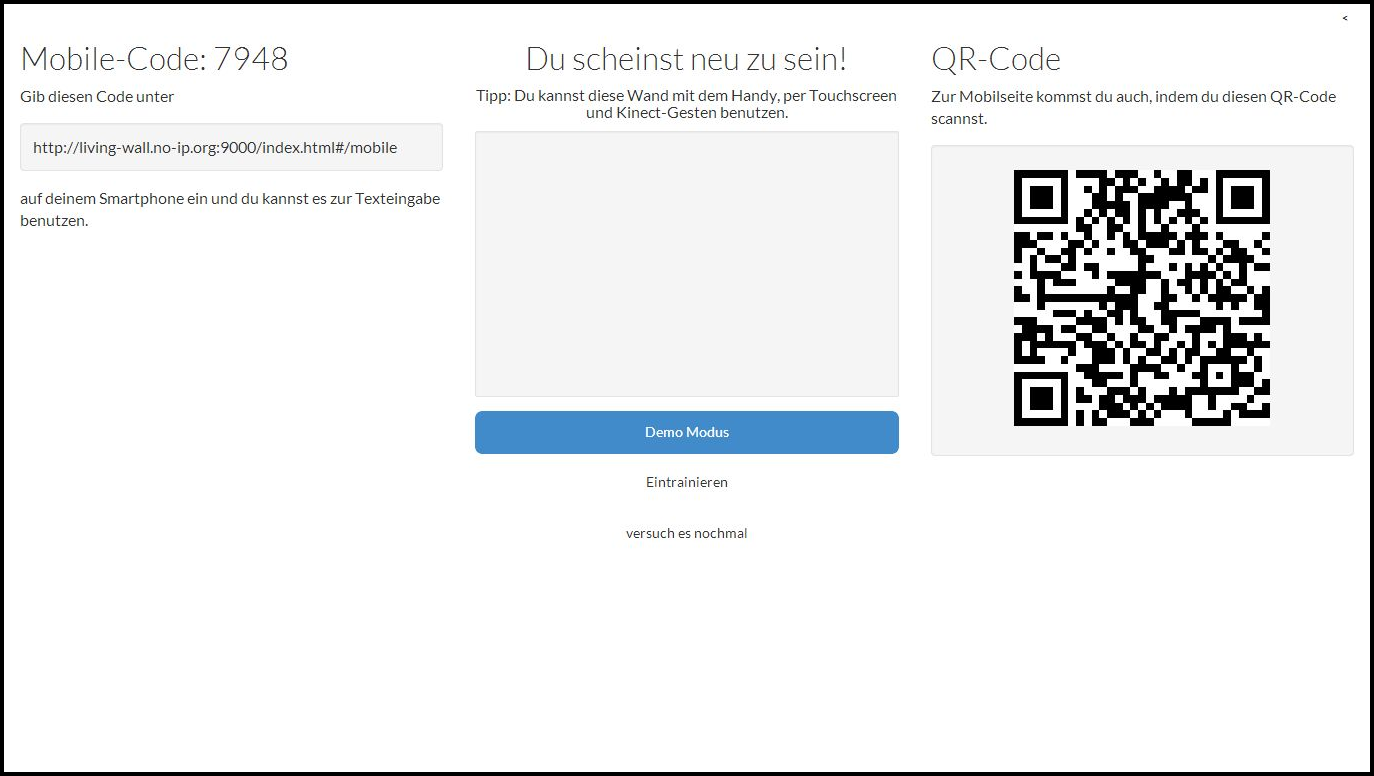
\includegraphics[scale=0.31]{UnknownUser}\\
		Es stehen nun drei Optionen zur Auswahl:
			\begin{itemize}
				\item \textbf{Demo Modus}\\
				Startet den Demo-Modus mit vorgespeicherten Demo-Daten, um dem Nutzer eine Möglichkeit zu geben, die Oberfläche der Living Wall auszuprobieren, ohne sich registrieren zu müssen. Die Bedienung ist unter dem Punkt 		\textit{Hauptansicht} erklärt.
				\item \textbf{Eintrainieren}\\
				Startet den Eintrainierungsprozess. Hierzu muss der Nutzer frontal zur Kamera stehen und in ihre Linse blicken. Es empfiehlt sich, den Kopf langsam und leicht zu neigen und drehen. Ein erfolgreiches Training führt in den Willkommensbildschirm für bekannte Nutzer (siehe \textit{Bekannter Nutzer}). Wenn die Kamera keine brauchbaren Bilder aufnehmen konnte, wird erneut der Bildschirm \textit{Unbekannter Nutzer} angezeigt, in dem der Prozess erneut gestartet werden kann.
				\item \textbf{versuch es nochmal}\\
				Wenn der Nutzer weiß, dass er schon in der eintrainiert ist und fälschlicherweise nicht erkannt wurde, kann er mit diesem Button einen neuen Erkennungsprozess starten.\\ \\
				\textit{Hinweis: Sollte die Erkennung nicht richtig funktionieren, empfiehlt es sich die Entfernung zur Kamera und die Beleuchtung zu variieren. Außerdem sollte der Nutzer stets in die Linse der Kinectkamera blicken.}
			\end{itemize}
		Um zwischen den Optionen zu wechseln, können die Gesten 'Tab nach oben' oder 'Tab nach unten' verwendet werden. Zum Bestätigen der Auswahl dient die 'Enter'-Geste.\\
Ausgewählt ist die jeweils \textbf{blau hinterlegte} Option! Im obigen Bild ist dies der Demo-Modus.\\ \\
Die Verwendung des Mobile- und des QR-Codes wird im Abschnitt \textit{Bekannter Nutzer} erklärt.
		\subsubsection{Bekannter Nutzer}
		Sollte der Nutzer von der Gesichtserkennung als unbekannt eingestuft werden, erscheint folgender Bildschirm:\\
		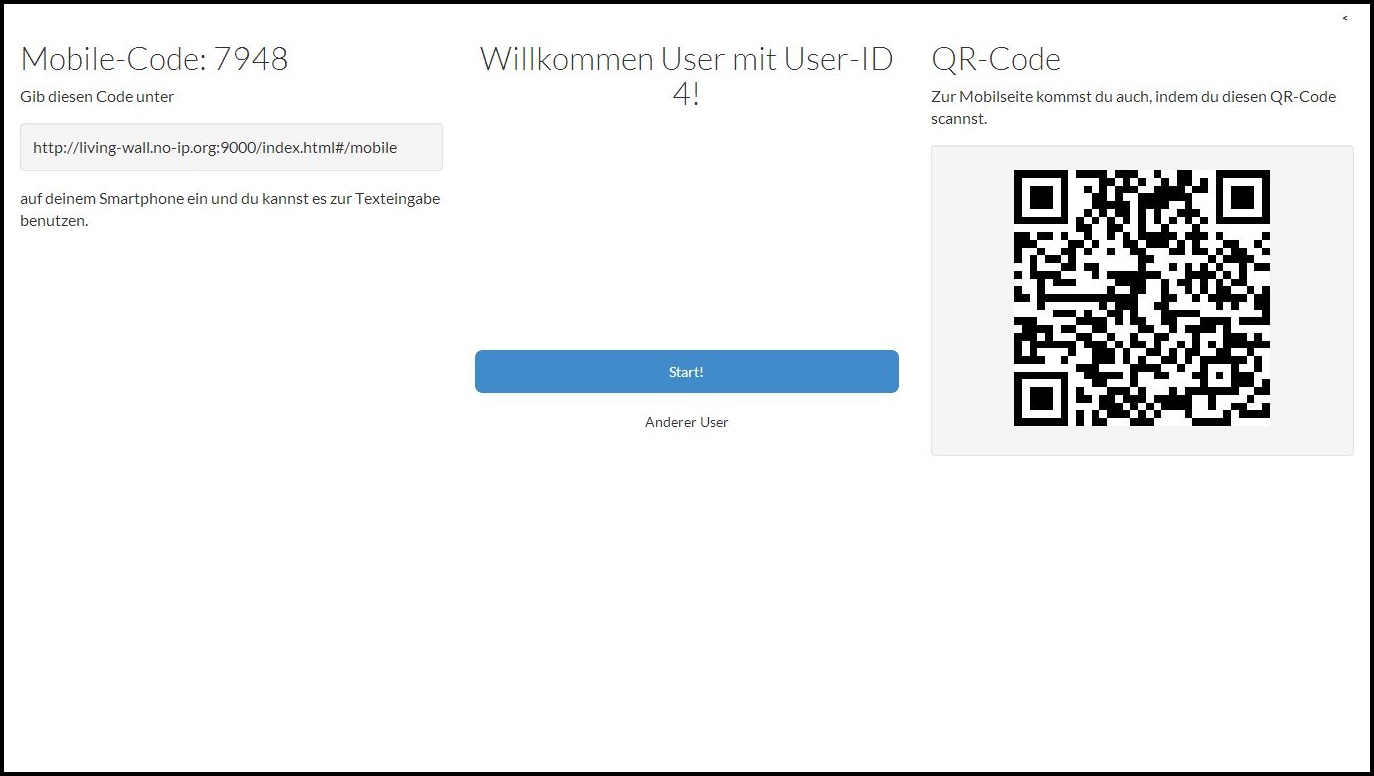
\includegraphics[scale=0.31]{Welcome}\\
		Es stehen nun zwei Optionen zur Auswahl:
			\begin{itemize}
				\item \textbf{Start!}\\
					Startet die individuelle Hauptansicht des erkannten Users mit seinen Widgets und Informationen. Die Bedienung ist im Abschnitt \textit{Hauptansicht} erklärt.
				\item \textbf{Anderer User}\\
				Wenn der Nutzer als ein anderer Nutzer erkannt wurde, als er eigentlich ist, kann er mit diesem Button eine neue Erkennung starten, um richtig erkannt zu werden.\\
				\textit{Hinweis: Sollte die Erkennung nicht richtig funktionieren, empfiehlt es sich die Entfernung zur Kamera und die Beleuchtung zu variieren. Außerdem sollte der Nutzer stets in die Linse der Kinectkamera blicken.}
			\end{itemize}
		Um zwischen den Optionen zu wechseln, können die Gesten 'Tab nach oben' oder 'Tab nach unten' verwendet werden. Zum Bestätigen der Auswahl dient die 'Enter'-Geste.\\
Ausgewählt ist die jeweils \textbf{blau hinterlegte} Option! Im obigen Bild ist dies 'Start!'.\\ \\
Der auf dem Bildschirm sichtbare Mobile-Code dient dazu, sein Smartphone mit der Wand zu verbinden, um mit ihm Eingaben machen zu können. Das genaue Verfahren und die Optionen zur Nutzung der Living Wall mit dem Smartphone werden im Abschnitt 	\textit{2.2.3 Bedienung mit dem Smartphone} behandelt.

		\subsubsection{Hauptansicht}
		Die Hauptansicht ist das Herzstück der Living Wall. In ihr bekommt der Nutzer seine persönlichen Informationen, Neuigkeiten wie News und Mails, Kalendereinträge, Todos und Meldungen aus sozialen Netzwerken, in denen er regsitriert und über die Living Wall angemeldet ist, in verschiedenen Widgets angezeigt:\\
		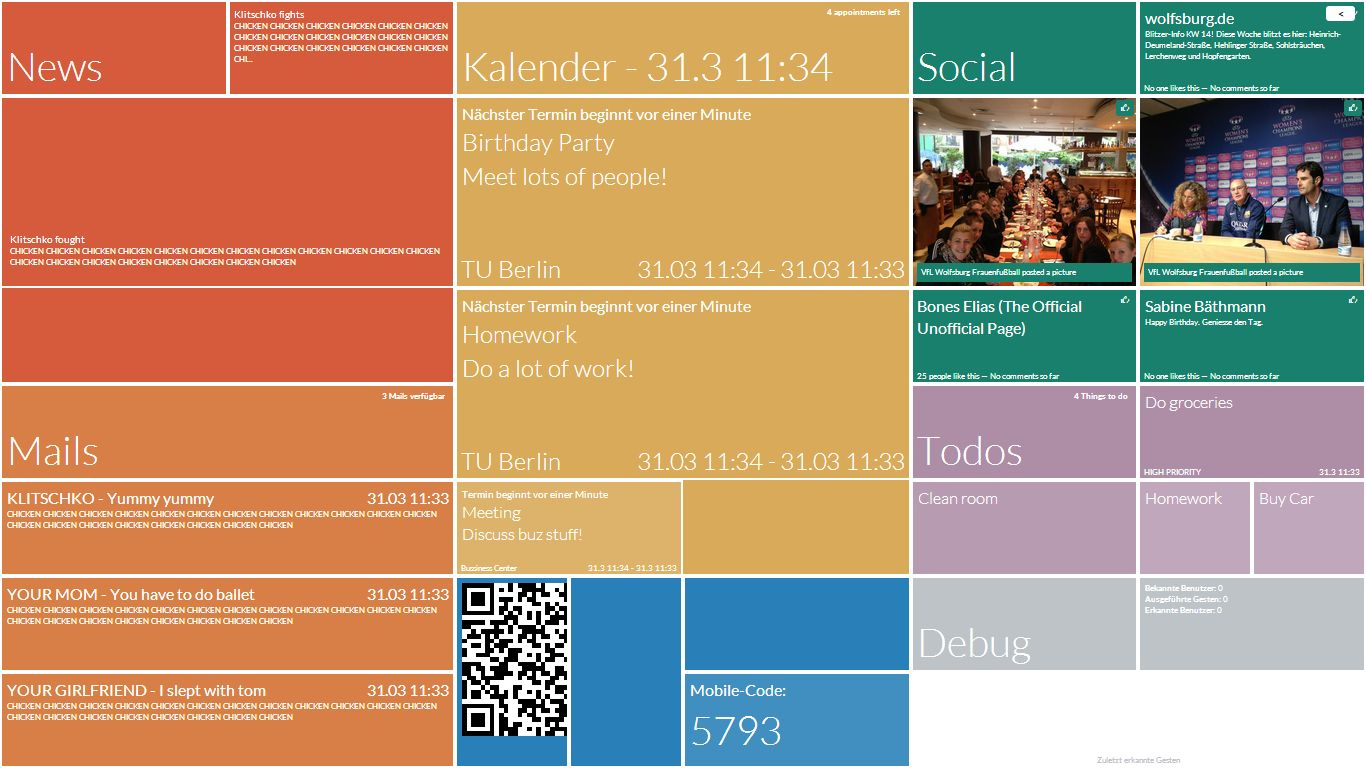
\includegraphics[scale=0.31]{Main}\\ \\
		\textit{Hinweis: Damit das Kalender- und das Mail-Widget Daten anzeigen, müssen die Google-Accountdaten des Nutzers in der Datenbank der Living Wall hinterlegt werden. Diese können komfortabel mit dem Smartphone eingetragen werden. Um das Facebook-Widget nutzen zu können, muss der Nutzer sich bei Facebook einloggen und der 'Ambient Assisted Living'-Facebookapp den Zugriff auf seine Daten gestatten. Auch der Facebook-Login kann mit dem Smartphone vollzogen werden. Das Vorgehen ist unter 'Bedienung mit dem Smartphone' genauer erklärt.}\\ \\
		Die Widgets sind durch ihre verschiedene Farbgebung und die Bennenung in der ersten, oberen linken Kachel leicht identifizierbar. In der Hauptansicht stehen viele verschiedene Möglichkeiten der Interaktion zur Verfügung:
			\begin{itemize}
				\item \textbf{Menü öffnen}\\
				Für fast alle Aktionen ist es nötig, das Menü zu öffnen. Hierzu wird die Geste 'Menü öffnen' verwendet. Auf dem folgenden Bild ist das geöffnete Menü zu sehen:\\
				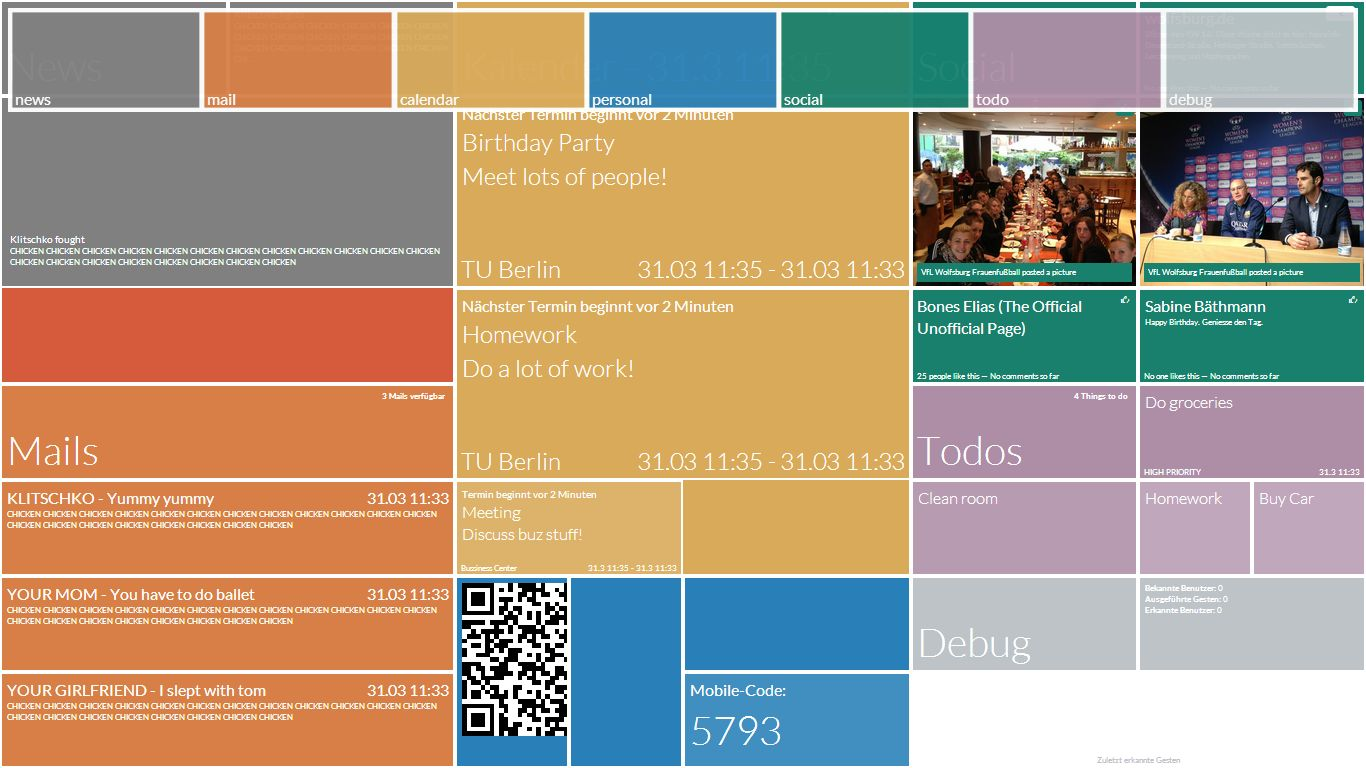
\includegraphics[width=\linewidth]{Menu1}\\
				Durch das geöffnete Menü kann mittels der Gesten 'Tab nach links' und 'Tab nach rechts' navigiert werden. Das ausgewählte Widget ist immer \textbf{grau hinterlegt}. Im obigen Bild ist es das 'News'-Widget.
				\item \textbf{Widget fokussieren}\\
				Wenn ein ausgewähltes Widget im Menü durch die 'Enter'-Geste angewählt wird, wird es in die Mitte des Bildschirms verlagert. Es kann auch mit nicht im Fokus liegenden Widgets gearbeitet werden. Der Übersicht halber empfiehlt es sich jedoch, das Widget von Interesse mit Hilfe des Menüs in die Mitte des Bildschirmes zu verschieben. Im obigen Bild ist das 'Kalender'-Widget das fokussierte Widget.
				\item \textbf{Einträge öffnen}\\
				Jedes Widget beinhaltet Kacheln mit Einträgen. Diese Einträge können ebenfalls über das Menü angewählt und dann geöffnet werden. Dazu muss im Menü mit 'Tab nach links' und 'Tab nach rechts' das Widget mit dem gewünschten Eintrag ausgewählt werden. Wählen wir zum Beispiel das 'Kalender'-Widget:\\
				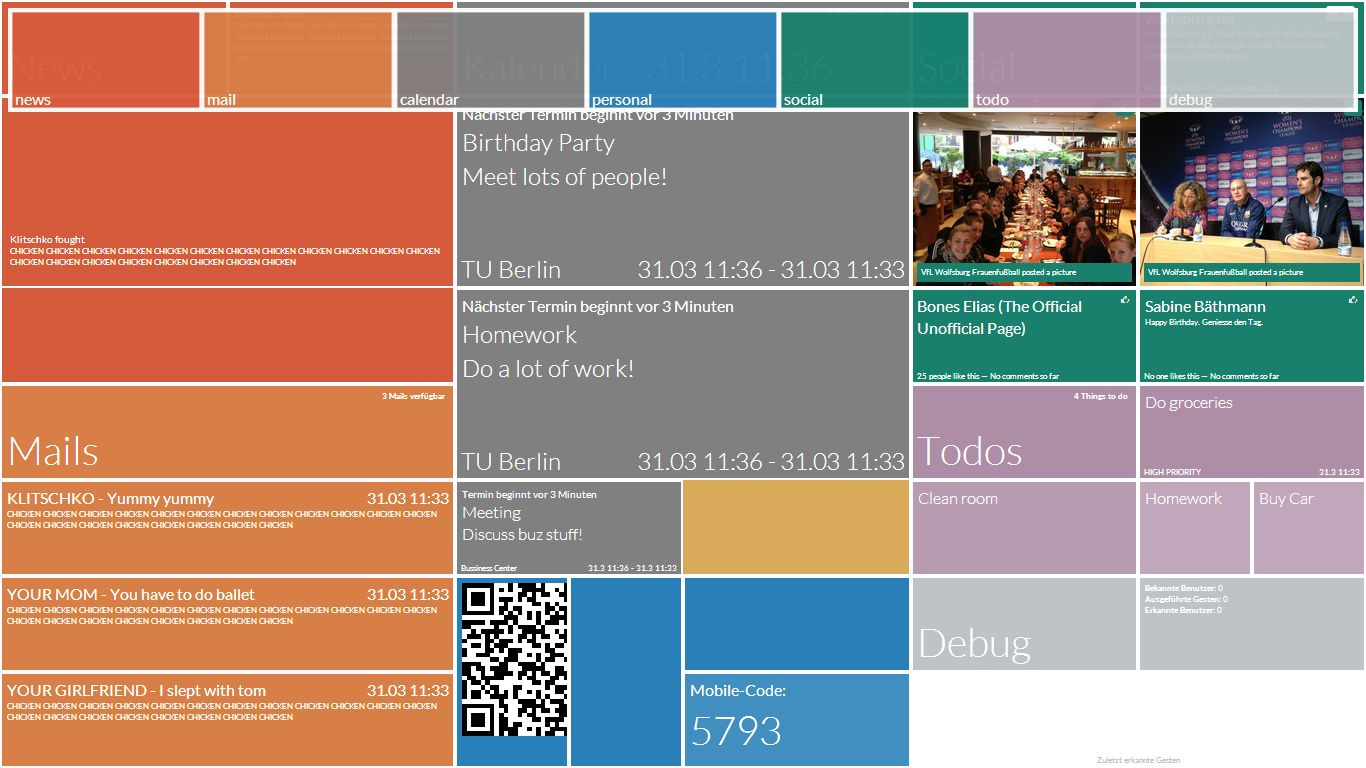
\includegraphics[width=\linewidth]{MenuSelect}\\
				Nun kann mit 'Tab nach unten' eine weitere Menüebene geöffnet werden. In dieser kann wieder mit 'Tab nach links' und 'Tab nach rechts' zwischen den Einträgen des Widgets gewechselt werden. Das jeweils ausgewählte Widget ist \textbf{grau hinterlegt}! Wird dieses nun mit der 'Enter'-Geste bestätigt, öffnet sich ein Popover zu dem angewählten Eintrag, das mehr Informationen enthält und je nach Widget die Möglichkeit zur Bearbeitung bzw. zum Löschen des Eintrags bietet:\\
				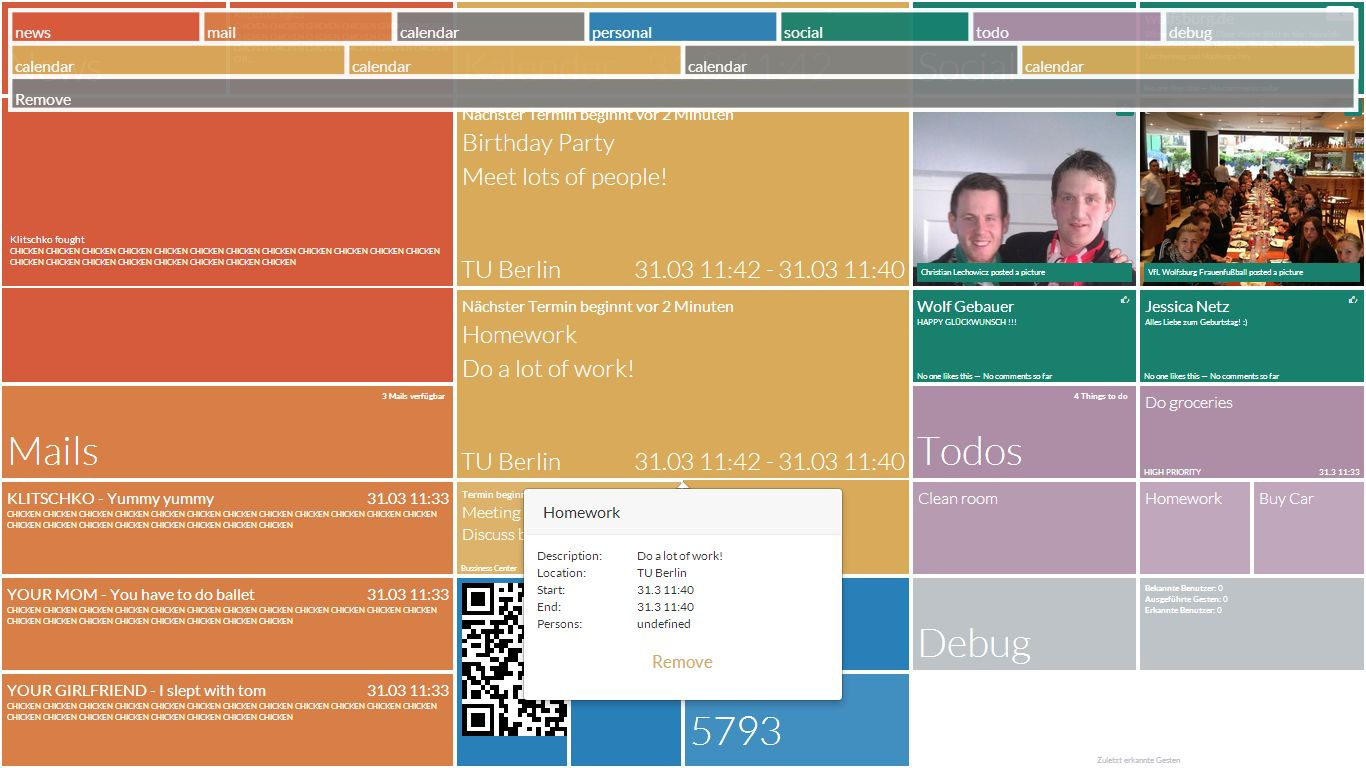
\includegraphics[width=\linewidth]{Popover}\\
				Die möglichen Optionen werden wie im Bild zu sehen in einer dritten Ebene des Menüs angezeigt. Hier ist dies nur das Entfernen des Eintrags. Dieser müsste wiederum mit der 'Enter'-Geste bestätigt werden.
				\item \textbf{Menü verlassen}\\
				Das Menü kann durch die 'Escape'-Geste komplett geschlossen werden. Mit 'Tab nach oben' und 'Tab nach unten' wird zwischen den verschiedenen Ebenen des Menüs gewechselt. Befindet man sich in der ersten Ebene und verwendet 'Tab nach oben', schließt sich das Menü. Anderenfalls wird jeweils eine Menüebene nach oben navigiert. Die maximale Tiefe des Menüs ist drei. 'Tab nach unten' hat auf dieser Ebene keine Wirkung.
				\item \textbf{Neue Einträge anlegen}\\
				Das Anlegen neuer Einträge funktioniert am besten mit dem Smartphone und ist unter \textit{Bedienung mit dem Smartphone} erklärt. Der Dialog kann allerdings auch per Gestensteuerung geöffnet und danach mit einem gekoppelten Smartphone oder per Touchscreen ausgefüllt werden. Dazu wird zuerst das Menü geöffnet und mit 'Tab nach links' und 'Tab nach rechts' das entsprechende Widget ausgewählt. Mit 'Tab nach unten' muss nun die zweite Menüebene geöffnet und \textbf{die erste Kachel} mit dem Namen des Widgets mit 'Tab nach links' und 'Tab nach rechts' markiert werden:\\
				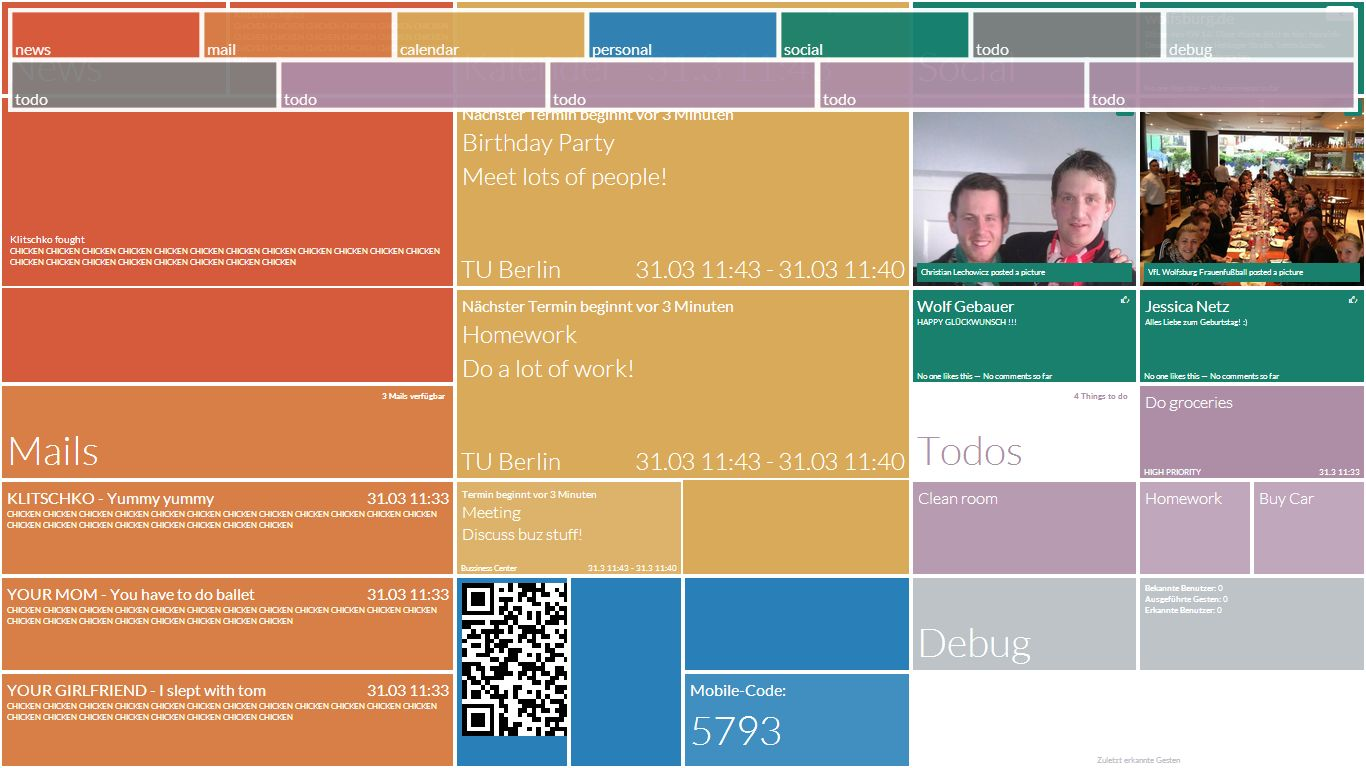
\includegraphics[width=\linewidth]{SelectTodo}\\
				Wird nun die 'Enter'-Geste verwendet, öffnet sich der Dialog zur Erstellung des neuen Eintrags auf der Living Wall selbst, auf der er per Touchscreen ausgefüllt werden kann, und auf dem gekoppelten Smartphone, insofern eines verbunden ist:\\
				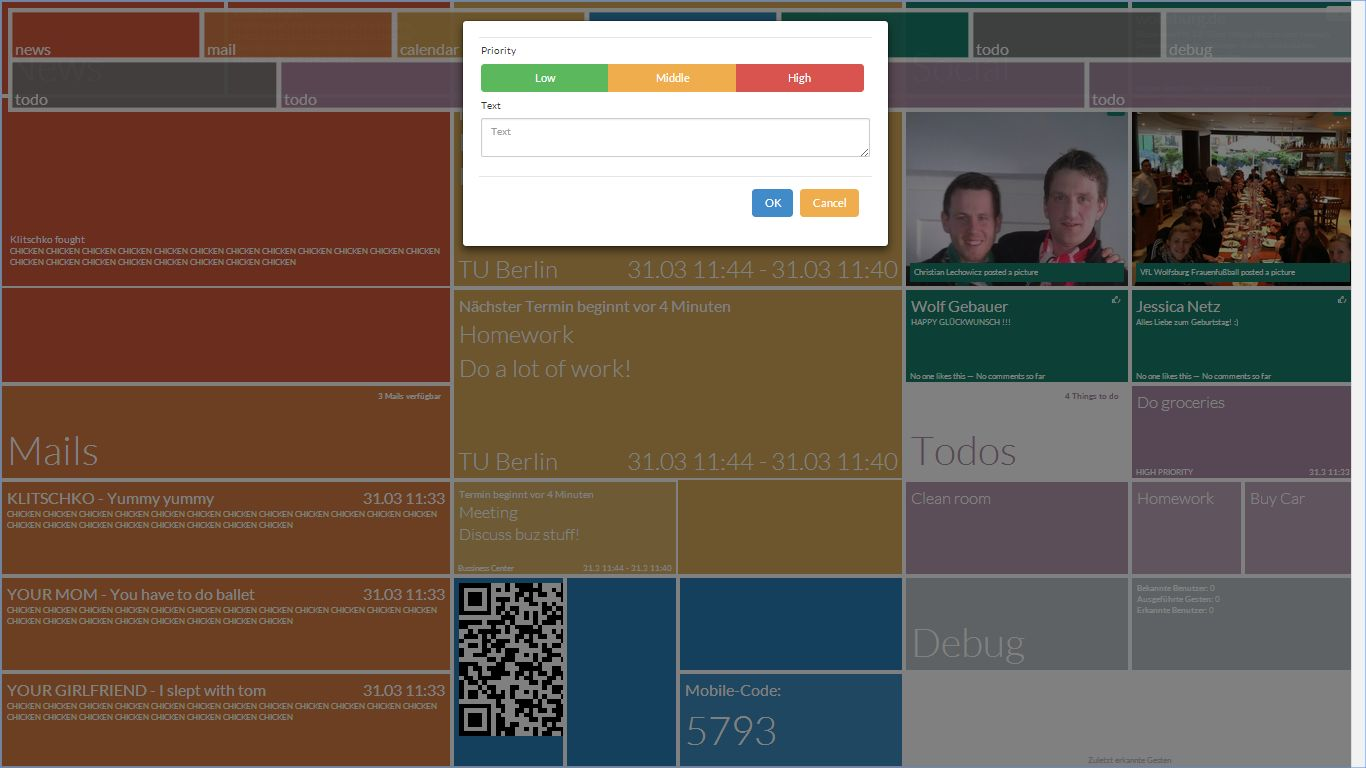
\includegraphics[width=\linewidth]{CreateTodo}\\
				Nachdem die neuen Daten eingetragen wurden, kann der Eintrag entweder mit 'OK' angelegt oder mit 'Cancel' verworfen werden.
			\end{itemize}

		\subsection{Mehrere Nutzer}
		Die Living Wall kann bis zu fünf Personen gleichzeitig erkennen und von diesen mit Gesten gesteuert werden. Die Gestensteuerung wird bei größerer Anzahl an Nutzern allerdings erheblich Fehleranfälliger. Daher sollte der Großteil der erkannten Personen die Gestenerkennung für sich selbst mit der 'Gestenerkennung ein-/ausschalten'-Geste blockieren.
		\subsubsection{Mindestens ein bekannter Nutzer}
		Wenn ein Nutzer von der Living Wall erkannt wird, kann er von seinem Willkommensbildschirm oder aus der Hauptansicht der Einzelnutzung heraus mit der 'User-Auswahl anzeigen'-Geste die Nutzer-Auswahl-Seite öffnen, auf der die sich im Blickfeld der Kinectkamera befindenden Nutzer angezeigt werden. Mit 'Tab nach links', 'Tab nach rechts' und 'Enter' kann dann ein User ausgewählt werden, der entweder auf seinen Willkommensbildschirm kommt (siehe \textit{Bekannter Nutzer}) oder auf den Bildschirm eines neuen Benutzers (siehe \textit{Ubekannter Benutzer}).\\
		Auf diesen Bildschirmen können sich unbekannte User nun eintrainieren, neu erkennen oder ihre Widgets anzeigen lassen.
		Sollten sich zwei bekannte Nutzer vor der Wand befinden, kann mit der 'Social-Graph-Ansicht öffnen'-Geste der Social-Graph geöffnet werden, welcher Gemeinsamkeiten der beiden Personen übersichtlich darstellt:\\
		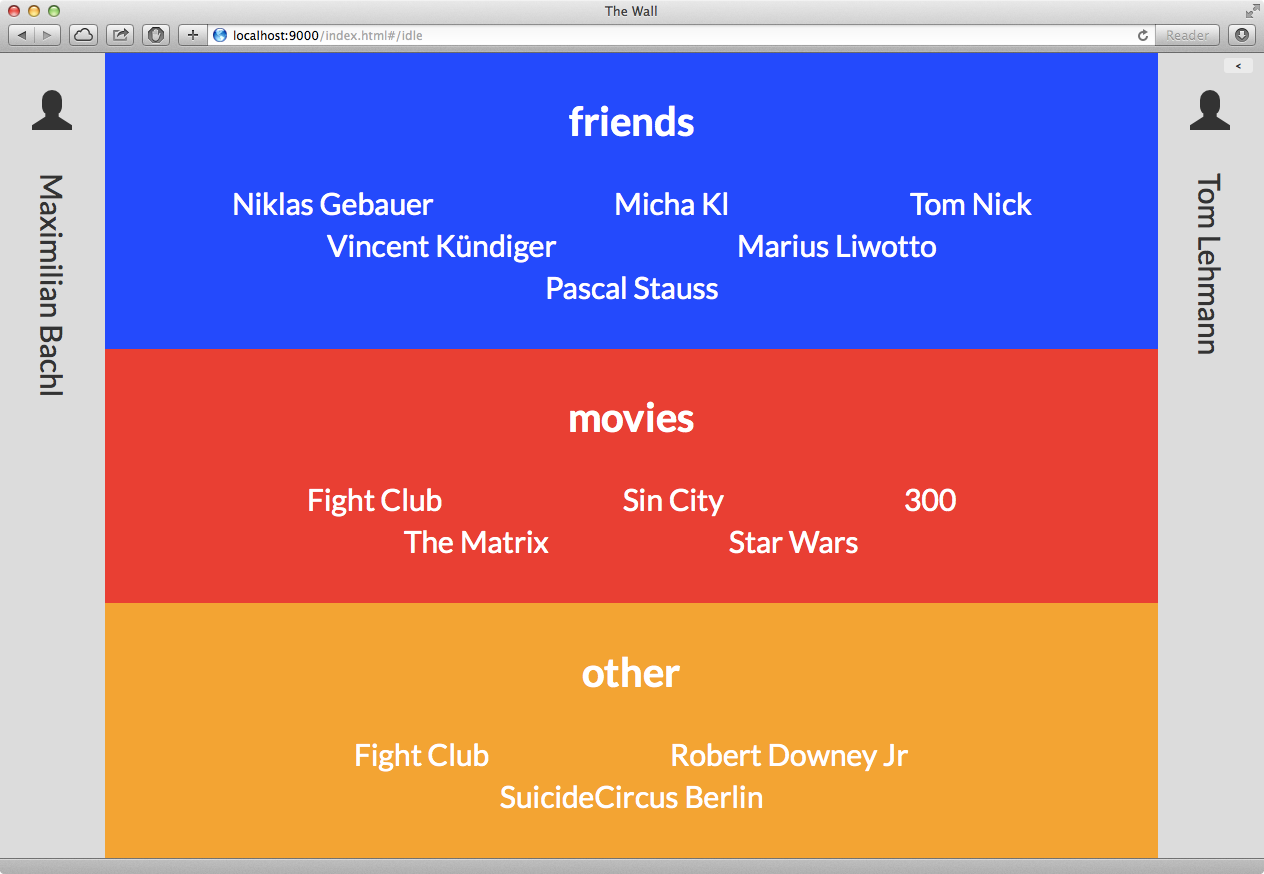
\includegraphics[width=\linewidth]{socialgraph}\\
		Sollte ein bekannter Nutzer sich auf seiner Willkommensseite oder in der Hauptansicht befinden, wird eine kleine Meldung am unteren Bildschirmrand eingeblendet, sobald ein zweiter bekannter Nutzer das Bild betreten hat und der Social-Graph geöffnet werden kann:\\
		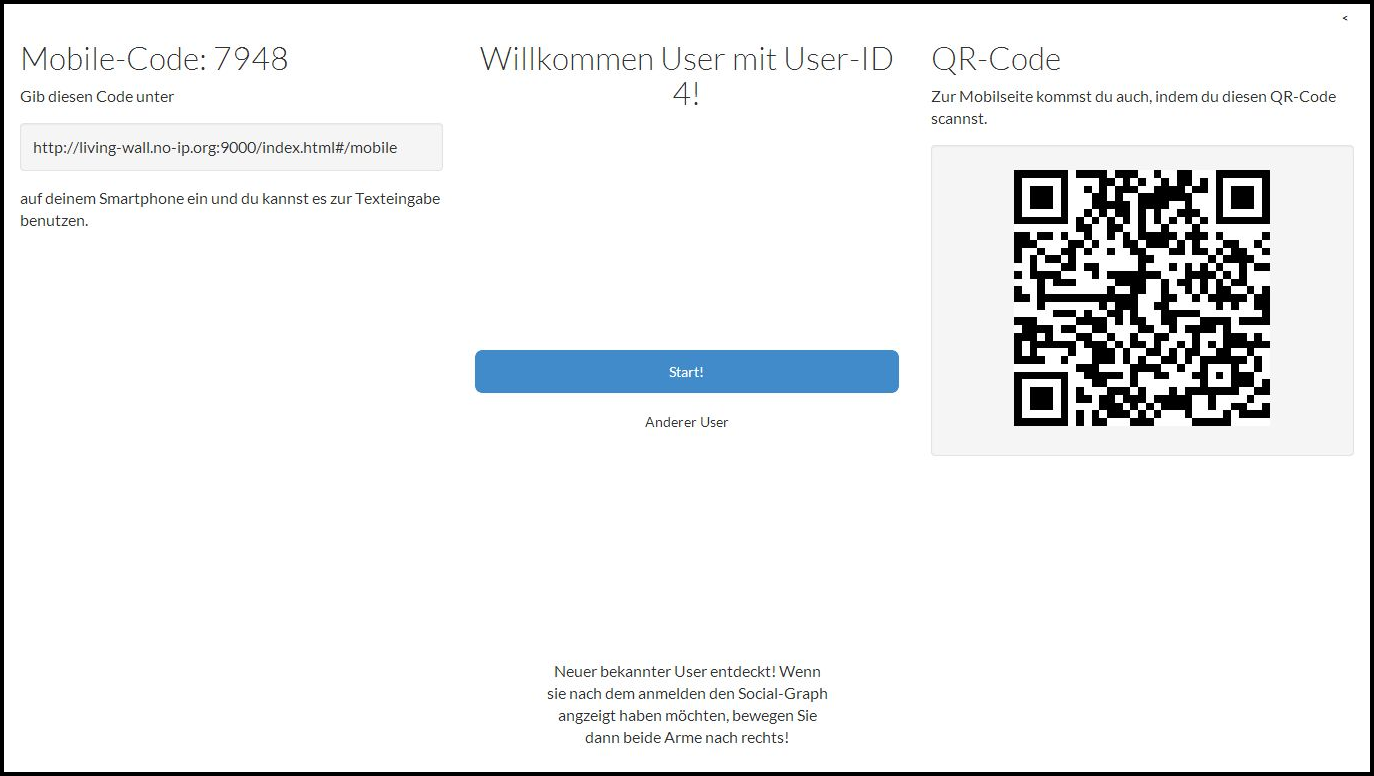
\includegraphics[width=\linewidth]{NewUser}
		\subsubsection{Nur unbekannte Nutzer}
		Wie im Fall von mindestens einem bekannten Nutzer, kann mit Hilfe der 'User-Auswahl anzeigen'-Geste die Nutzer-Auswahl-Seite geöffnet werden, um wie bereits beschrieben den aktiven Nutzer auszuwählen. Allerdings wird sich nur die Seite für Unbekannte Nutzer öffnen, auf der diese sich eintrainieren oder neu erkennen lassen können (siehe \textit{Ubekannter Benutzer}). Außerdem können sie die Living Wall im Demo-Modus testen. Der Social-Graph lässt sich allerdings nur mit bekannten Nutzern aufrufen.

		\subsection{Bedienung mit dem Smartphone}
		Das Smartphone ist ein mächtiges und komfortables Eingabegerät für die Nutzung der Living Wall. Im Folgenden ist die Bedienung der Living Wall mit dem Smartphone genauer beschrieben. Um eine einwandfreie Anzeige zu gewährleisten, empfehlen wir die mobile Version des Browsers 'Chrome' auf dem Smartphone zu installieren.\\ \\
		\textit{Hinweis: Um sich mit der Living Wall verbinden zu können, muss das Smartphone mit dem Internet verbunden sein.}
		\subsubsection{Kopplung mit der Living Wall}
		Um das eigene Smartphone mit der Living Wall zu verbinden, gibt es zwei Möglichkeiten.
			\begin{itemize}
				\item \textbf{Website aufrufen und Mobile-Code eingeben}\\
				Wie im Abschnitt \textit{Bekannter Benutzer} zu sehen, gibt es auf der Willkommensseite oben links eine URL. Diese kann im Browser des Smartphones ganz einfach eingegeben und geladen werden. Es öffnet sich die mobile Seite der Living Wall:\\
				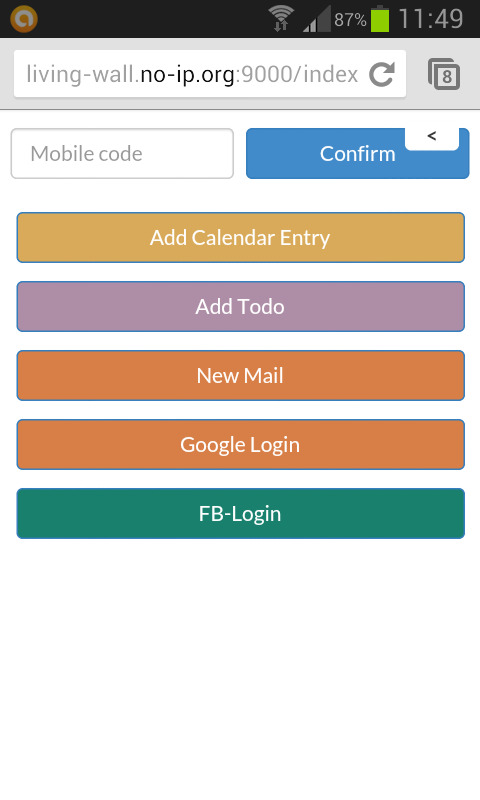
\includegraphics[scale=0.3, trim=0 8cm 0 0]{mobile}\\
				In dem Feld 'Mobile code' muss der vierstellige Zahlen-Code eingegeben werden, welcher sich oben links auf der Willkommensseite befindet (siehe \textit{Bekannter Benutzer}) und danach mit einem Druck auf 'Confirm' bestätigt werden. Danach ist das Smartphone erfolgreich mit der Living Wall gekoppelt. \\
				\item \textbf{QR-Code scannen}\\
				Alternativ kann mit einem beliebigen QR-Code-Scanner der rechts oben auf der Willkommensseite abgebildete QR-Code gescannt und die entschlüsselte URL im Browser geöffnte werden. Der Mobile-Code wird bei dieser Methode automatisch eingetragen. Nach dem Laden der Seite ist das Smartphone also automatisch gekoppelt und bereit zur Interaktion mit der Living Wall.
			\end{itemize}
		\subsubsection{Anlegen von Einträgen}
		Der Dialog zum Anlegen von Einträgen kann wie im Abschnitt \textit{Hauptansicht} beschrieben geöffnet werden. Wenn ein Smartphone mit der Living Wall verbunden ist, öffnet sich auch auf diesem der Dialog. Für Kalendereinträge, Todos und Mails kann der Dialog auch direkt über die Buttons auf dem Smartphone geöffnet werden. Er erscheint auch dann sowohl auf der Living Wall als auch auf dem Smartphone. Das folgende Bild zeigt beispielsweise den Dialog zum Anlegen von Todos auf dem Smartphone:\\
		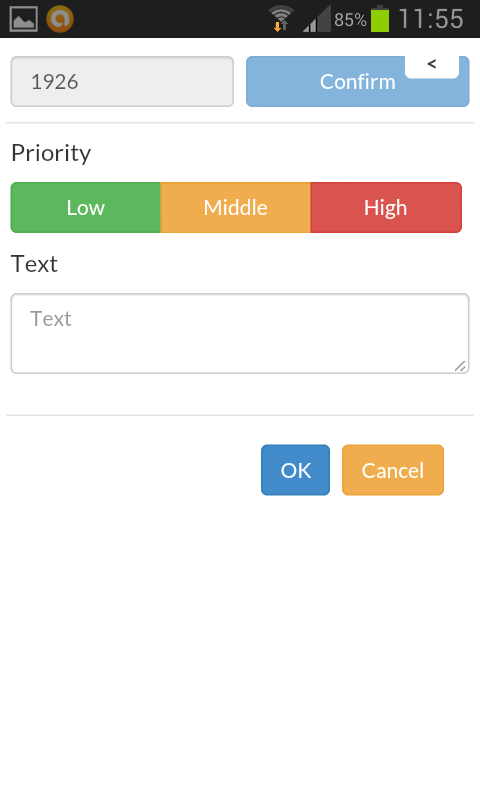
\includegraphics[scale=0.3, trim=0 8cm 0 0]{createTodoMobile}\\
		Die Daten, die auf dem Smartphone eingegeben werden, werden in Echtzeit an die Living Wall übertragen. Sobald alle erforderlichen Felder ausgefüllt sind, kann der Eintrag mit 'OK' entweder angelegt oder mit 'Cancel' verworfen werden. Das Smartphone kehrt darauf hin auf die normale Mobilseite zurück, die Living Wall zeigt die Hauptansicht.
		\subsubsection{Facebook-Login}
		Sobald das Smartphone wie oben unter \textit{Kopplung mit der Living Wall} beschrieben verbunden wurde, kann der Nutzer sich über den 'FB-Login'-Button bei Facebook einloggen.\\
Es öffnet sich der Standard-Login-Dialog von Facebook. Sobald die Mailadresse und das Passwort, mit denen der Nutzer bei Facebook registriert ist, erfolgreich eingegeben wurden, kann das Facebook-Widget der Living Wall die Daten des Nutzers anzeigen.\\ \\
		\textit{Hinweis: Beim ersten Login bei Facebook mit der Living Wall, muss der Nutzer der 'Ambient Assisted Living'-Facebookapp den Zugriff auf seine Daten gewähren. Ohne diese Erlaubnis kann das Facebook-Widget keine Daten anzeigen. Die Erlaubnis kann jederzeit im Nachhinein in Facebooks App-Verwaltung entfernt werden. Sollte sich der Nutzer danach erneut mit der Living Wall bei Facebook einloggen, muss die Erlaubnis weider erteilt werden, falls das Facebook-Widget benutzt werden soll.}
		\subsubsection{Google-Login}
		Sobald das Smartphone wie oben unter \textit{Kopplung mit der Living Wall} beschrieben verbunden wurde, kann der Nutzer über den 'Google Login'-Button seine Google-Daten in der Datenbank der Living Wall hinterlegen. Mit diesen werden dann zum Beispiel die Mails und Kalenderdaten des Google-Accounts in die Datenbank geladen.\\
Nach dem Drücken des 'Google Login'-Buttons öffnet sich ein Dialog, in dem lediglich die Googlemail-E-Mail-Adresse und das dazugehörige Passwort eingegeben und mit 'OK' bestätigt werden müssen. Dieser Vorgang braucht im Gegensatz zum Facebook-Login nur einmalig vom Nutzer durchgeführt werden.

\chapter{Projektbericht}
	In diesem letzten Kapitel der Projektdokumentation möchten wir noch einmal auf besondere Herausforderungen und Leistungen eingehen, sowie eine allgemeine Reflexion des Projekts durchführen.\\\\
	Ziel des Projekts war es, eine "`Living Wall"' zu erstellen, welche den Nutzer in verschiedenen Szenarien unterstützt und Informationen bereitstellt. Unsere Aufgabe war es dabei, für die Visualisierung sowie die Möglichkeit der Texteingabe zu sorgen. Die Realisierung der Aufgabe sollte bis zum Ende des Semesters erfolgen und die Projektfortschritte während zwölf, in wöchentlichem Abstand stattfindenden Terminen, den anderen Projektteilnehmern präsentiert werden. Schlussendlich sollte noch eine Dokumentation, bestehend aus Entwickler- und Userhandbuch, sowie ein Projektbericht erstellt werden.
	
\section{Frontend-Entwicklung}
	Die Aufgabenstellung wirkte sehr reizvoll und wir begannen damit, uns Gedanken über die Möglichkeiten der Darstellung zu machen. Wir entschieden uns dafür, die Darstellung der Informationen in "`Widgets"' zu realisieren. Ein Widget ist eine unabhängige Funktionseinheit, die gemeinsam mit anderen Widgets zur Gesamtanwendung komponiert wird. Ein Beispiel für ein Widget wäre etwa unser Kalender. Neben dem Kalender gibt es z.B. auch noch das Facebook-Widget. All diese Widgets gemeinsam sind für das Gesamterlebnis der Anwendung verantwortlich. Das hat den Vorteil, dass man einen modularen Aufbau hat und eventuell später erforderliche Funktionalität einfach hinzufügen kann, bzw. in bestimmten Anwendungsfällen nicht benötigte Komponenten ausblenden kann, ohne andere Teile der Anwendung zu beeinträchtigen. Auf dieser Basis arbeiteten wir einige Designentwürfe aus, entschieden uns für geeignete Software und erstellten eine passende Projektstruktur. Bei der Wahl der Software waren insbesondere zwei Faktoren von besonderer Signifikanz. Zum einen sollten wir Jiac zur Kommunikation mit anderen Gruppen einsetzen, sodass unser Backend Java unterstützen musste und zum anderen wollten wir, dass die Vorteile unseres Widgetkonzepts sich auch im Code äußern. Deshalb entschieden wir uns dafür, im Backend Play einzusetzen und im Frontend mit AngularJS zu arbeiten, da die Angular Directives unsere Anforderungen in besonderem Maße erfüllen würden.\\\\
	Bei den Überlegungen zum Design unseres Interfaces war es vonnöten eine Vielzahl von Faktoren zu berücksichtigen, die wir aber zunächst selbst herausfinden mussten und über deren Wichtigkeit wir zum Teil ausführlichst nachgedacht und diskutiert haben, da wir kaum Vorwissen über Interfacedesign mitbrachten.\\\\
	Die nächste große Herausforderung für uns war, wie man unser Interface möglichst intuitiv und sinnvoll bedienen kann. Ein Cursor wurde aus verschiedenen Gründen ausgeschlossen, also überlegten wir uns verschiedene Möglichkeiten die Wand über anders geartete Gesten zu steuern und haben uns schließlich für "`Vier-Wege-Tabbing"' in Kombination mit der Darstellung eines Menüs zur Unterstützung der Navigation und Interaktion entschieden. Die visuelle Darstellung des Menüs war recht komplex, da wir das Menü generisch implementieren wollten, um es somit unabhängig von der Anzahl der dargestellten Widgets zu gestalten.\\\\
	Weil wir ohnehin eine Mobilseite für die Texteingabe erstellen mussten, welche die Möglichkeit bieten sollte, Texteingaben im Interface der Wall mit Live-Feedback via Smartphone zu realisieren, haben wir uns dafür entschieden, den Inhalt der Mobilseite dynamisch zu updaten. Das heißt, dass sich die Anzeige auf dem Mobilgerät selbstständig ändert, wenn auf der Wall eine Aktion ausgeführt wurde, welche das Mobilgerät erforderlich macht. Wird die Aktion über das Smartphone oder über die Wall beendet, kehrt die Mobilseite automatisch in einen Zustand zurück, in dem die Kernfeatures der Wall (z.B. Mail erstellen) direkt mit einem Knopfdruck ausgelöst werden können und sich der Zustand auf dem Mobilgerät dementsprechend anpassen würde. Wir haben also für gekoppelte Geräte und die Wall einen asynchrone Echtzeitkommunikationskanal aufgebaut, um dem User das bestmögliche Feedback, direktes visuelles Livefeedback, zu ermöglichen. Um die Orientierung des Nutzers zu vereinfachen, haben wir bei der Implementierung darauf geachtet, dass sowohl das Fenster auf der Wall, als auch der auf dem Mobilgerät angezeigte Dialog das selbe Template benutzen und sich somit, bis auf einige bildschirmgrößenspezifische Unterschiede, visuell gleichen und die Anpassung und Wartung des Codes vereinfacht wird.\\\\
	Zuletzt sei zum Frontend noch der Social-Graph erwähnt. Wie vorhin schon erläutert ermöglicht er nach der Erkennung die Darstellung von Gemeinsamkeiten, damit User möglicherweise schon ein Gesprächsthema oder gemeinsames Interesse zu Beginn der Wall-Interaktion erkennen.\\
	Ursprünglich war für den Social-Graph eine Graph-Darstellung angedacht. Diese hat sich aber im Laufe des Entwurfsprozesses als nicht so praktikabel wie ursprünglich gedacht herausgestellt, da die Anzahl an Gemeinsamkeiten der User kleiner war als vermutet und der Graph somit meistens nur eine Hand voll Knoten besaß und kaum informativ war.\\
	Darum wurde dann eine tabellarische Darstellung gewählt. Ein Vorteil ist, dass sich bei dieser Form die Kategorien der angezeigten Daten problemlos erweitern lassen. Hierzu sind kaum Änderungen im Backend erforderlich.\\ 
	Eine weitere Änderung ist, dass ursprünglich bis zu 5 Leute für den Social-Graph geplant waren. Nach Tests stellte sich aber heraus, dass mit zunehmender Anzahl an Personen, die Ladezeiten (um die Daten von Facebook zu laden und sie anschließend zu analysieren und darzustellen) unannehmlich groß wurden.\\
Daher wäre hier für eine potentielle Weiterentwicklung unserer Arbeit ein guter Ansatzpunkt. Allerdings müssten dafür auch die Funktionalitäten anderer Gruppen erweitert werden. Um den Graph für fünf Personen sinnvoll nutzbar zu machen, sollten mehr Daten zu jedem User aus mehr Quellen frühzeitig in der Datenbank sortiert und gespeichert werden. Erst dann kann eine nützliche Visualisierung in Form einer Graph-Darstellung stattfinden.

\section{Backend-Entwicklung}
	Im Backend entschieden wir uns wie vorhin schon kurz erwähnt für das Play-Framework. Diese Software ermöglichte uns große Performance und stellte uns auch alle benötigten Funktionen ohne Umwege zur Verfügung. Besondere Erwähnung verdienen hier die "`Websockets"'.\\
	Bei dieser Technologie wird es ermöglicht, auch direkt im laufenden Betrieb vom Server Daten für die Website nachzuladen. Das ganze ist sehr ähnlich zum älteren "`AJAX"' , mit dem Unterschied, dass bei der Verwendung von Websockets auch der Server spontan Daten an den Client senden kann, ohne dass der Client dies vorher explizit gefordert hat.\\
	Somit ermöglichten uns Websockets, dass die Inhalte der Widgets, wie etwa News oder Facebookdaten, live vom Server nachgeladen werden können. Auch ohne Aktualisierung der Website ist es somit potentiell möglich, die Daten über mehrere Tage hinweg aktuell zu halten.

\section{Schlussfolgerungen}
Allgemein kann man festhalten, dass die Motivation für das Projekt in unserer Gruppe sehr groß war und wir besonders zu Beginn sehr begeistert waren. Darum starteten wir auch zügig mit der Entwicklung des Frontends, welches schon sehr schnell konkrete Formen annahm.\\
%ACHTUNG: der nächste Absatz ist Bullshit.
Ein Problem hierbei war, dass die benutzten Technologien sowohl auf Frontend- als auch auf Backend-Seite den meisten Gruppenmitgliedern zu Beginn nicht geläufig waren. Das ist an sich kein Problem, da unsere Erfahrung mit derartigen Webprojekten natürlich als Studenten beschränkt ist. Wir unterschätzten aber den Aufwand, den die Einarbeitung erfordert. Besonders Angular-JS ist sehr mächtig, komplex und facettenreich, wodurch eine lange Einarbeitungszeit notwendig wurde. Bezüglich der Entwicklungsarbeiten hätten wir den Einarbeitungsaufwand also großzügiger schätzen sollen.\\\\
Die Kommunikation mit den anderen Gruppen war generell sehr harmonisch und die Arbeitsatmosphäre war produktiv-angespannt, aber stets höflich und hilfsbereit. Als einzigen Missstand kann man hier die mangelnde Kommunikation anführen. Manchmal schien es, als ob die Gruppen aneinander vorbeiarbeiten würden, da einfach nicht genug Absprachen getroffen wurden. Wir vermuten, dass dies der bis jetzt mangelnden Erfahrung in großen Gruppenarbeiten der Beteiligten zu schulden ist.\\
Wie auch bezüglich der Entwicklungsarbeiten zuvor, stellt man schnell fest, dass die mangelnde Erfahrung in mancherlei Hinsicht ein Problem darstellte, das aber in gewisser Weise natürlich gegeben war, da die meisten von uns Bachelor-Studenten im 4.~bis 6.~Semester sind.\\\\

	TODO: Herausforderungen/Leistungen im Backend und ggf. Social-Graph oder andere Dinge im Frontend, die mir noch nicht eingefallen sind


\end{document}
